% ----------------------------------------
%
% LaTeX Article Template for CUED Reports
% Jon Sowman - 2009
% jon@hexoc.com
% 
% ----------------------------------------
% Set up the document class for an article
\documentclass[11pt,twocolumn]{article}

% Import the required packages for latex
\usepackage{appendix}

% This packages permits using $ \therefore $
\usepackage{amssymb}
\usepackage{graphicx}

% This package allows the use of $ \text{} $
\usepackage{amsmath}
\usepackage{savetrees}

% The document title and author
\title{SB3 - Logic Analyser\\Datasheet}
\author{Jon Sowman\\Selwyn College}

% Begin the document
\begin{document}
    \maketitle
	
    \begin{figure}
    \centering
    
\includegraphics[height=3cm]{blank}
    \caption{Logic Analyser}
    \label{fig:la}
    \end{figure}

\section{Specification}
    \begin{itemize}
        \item High speed sampling up to 250kHz with input overvoltage
            protection.
        \item Compact and low cost
        \item Bus powered, no external power supply required
        \item Inbuilt hysteresis via Schmitt triggers on all input channels.
        \item Fully featured user interface allowing configuration of the
            analyser and displaying of the results
    \end{itemize}

\section{Usage}
\subsection{Setting Up}
    Plug the logic analyser into a spare USB port on your computer and open the
    \texttt{LogicAnalyser.exe} software on your computer. The central indicator
    should turn green indicating that the analyser has been detected and
    communications are in progress. Disconnecting the analyser will result in
    this indicator turning red (see figure \ref{fig:ui-config}). 
    If this happens, reconnect the analyser and
    click the \texttt{Reconnect} button.

    \begin{figure}
    \centering
    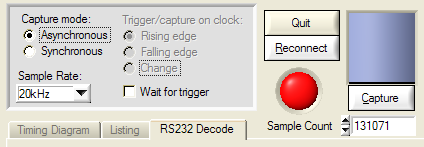
\includegraphics[height=3cm]{ui-config}
    \caption{Analyser configuration}
    \label{fig:ui-config}
    \end{figure}

\subsection{Configuration}
   The analyser is capable of operating in three modes: 
   \begin{itemize}
        \item Asynchronous non-triggered - takes the required number of
            captures at the required sample rate as soon as the
            \texttt{Capture} button is pressed.
        \item Asynchronous triggered - wait for the corresponding trigger on
            channel 0 and then starts sampling at the required sample rate up
            to the sample number.
        \item Synchronous - take samples on the rising, falling or changing
            edge of channel 0, as configured in the UI panel.
    \end{itemize}

    For all modes, the maximum number of samples can be set in the
    \texttt{Sample Count} text entry field, up to a maximum of $131,071$.

    Press the \texttt{Capture} button to configure the analyser and arm it.
    Capture will begin immediately in non-triggered modes or as soon as a
    trigger is received in triggered modes. The analyser must not be
    disconnected from the computer during the sampling procedure.

\subsection{Analysis}
    During sampling the blue progress bar will fill up, representing the
    progress of the analyser. When the progress bar reached the top, capture is
    complete and the data will automatically start being transferred to the PC
    for display and analysis.

    Once the blue progress bar reaches the bottom, transfer of data from the
    analyser to the PC is complete. At this point you may select one of the
    tabs in the display section to view the data, for example the timing
    diagram shown in figure \ref{fig:ui-timing}.

    To choose which section of the data is displayed, use the two sliders 
    underneath the display area. The left sets the window size and the right
    sets the position of the window within the captured data.

    You may turn off display of any or all channels using the checkboxes at the
    bottom of the display area. In addition you may use the \texttt{Display
    All} or \texttt{Display None} buttons to display all or no channels
    respectively.

    To decode RS232, choose the \texttt{RS232 Decode} tab followed by the
    channel you wish to decode and its baud rate. Press the \texttt{Decode}
    button to commence RS232 decoding of the channel.

    \begin{figure}
    \centering
    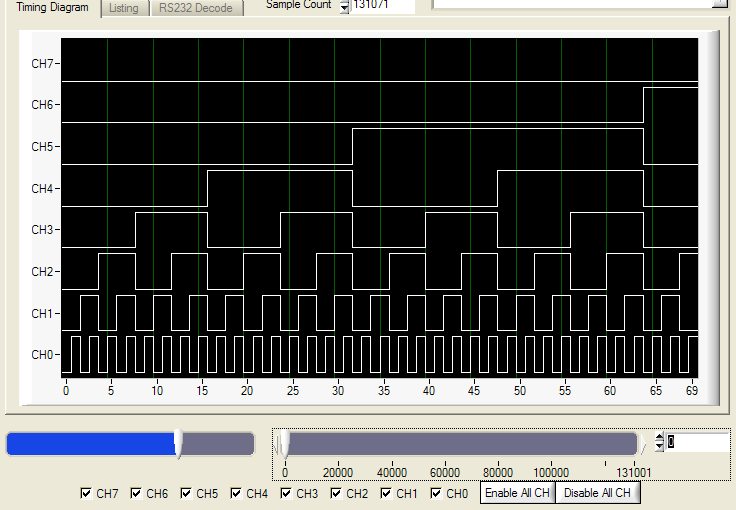
\includegraphics[height=4.8cm]{ui-timing}
    \caption{Analyser data display}
    \label{fig:ui-timing}
    \end{figure}
	
\end{document}
